\chapter{Charging Current and Choice of Gating Temperature in Ionic Liquid Gating\label{ch:Gating_T}}

%Appendices are just chapters, included after the $\backslash appendix$ command.
%
%\section{Switching Formats}
%When switching \texttt{printmode} on and off (see Section~\ref{sec:usage:options}), you may need to delete the output .aux files to get the document code to compile correctly. This is because the hyperref package is switched off for \texttt{printmode}, but this package inserts extra tags into the contents lines in the auxiliary files for PDF links, and these can cause errors when the package is not used.
%
%\section{Long Tables}
%
%Long tables span multiple pages. By default they are treated like body text, but we want them to be single spaced all the time. The class therefore defines a new command, $\backslash tablespacing$, that is placed before a long table to switch to single spacing when the rest of the document is in double spacing mode. Another command, $\backslash bodyspacing$, is placed after the long table to switch back to double spacing. Normal tables using \texttt{tabular} automatically use single spacing and do not require the extra commands.
%
%When the documentclass is defined with the `singlespace' option, these commands are automatically adjusted to stay in single spacing after the long table.
%
%Make sure there is always at least one blank line after the $\backslash bodyspacing$ command before the end of the file.
%
%Some times long tables do not format correctly on the first pass. If the column widths are wrong, try running the \LaTeX compiler one or two extra times to allow it to better calculate the column widths.
%
%If you want your long table to break pages at a specific point, you can insert the command $\backslash pagebreak[4]$, to tell \LaTeX that it really should put a page break there. $\backslash pagebreak[2]$ gives it a hint that this is a good place for a page break, if needed. If there's a row that really should not be broken across a page, use $\backslash \backslash *$, which will usually prevent a pagebreak. 
%
%\section{Booktabs}
%%The booktabs package is included to print nicer tables. See the package documentation~\cite{fear2005booktabs} for more details and motivation. Generally, all vertical lines are removed from the tables for a better visual appearance (so don't put them in), and better spacing and line thicknesses are used for the horizontal rules. The rules are defined as $\backslash toprule$ at the top of the table, $\backslash midrule$ in between the heading and the body of the table (or between sections of the table), and $\backslash bottomrule$ at the end of the table. $\backslash cmidrule$ can be used with the appropriate options to have a rule that spans only certain columns of the table.
%
%\section{Bibliography and Footnotes}
%
%The bibliography and any footnotes can also be single spaced, even for the electronic copy. The template is already setup to do this.
%
%Bibliography entries go in the .bib file. As usual, be sure to compile the \LaTeX code, then run BibTeX, and then run \LaTeX again.
%
%To cite websites and other electronically accessed materials, you can use the `@electronic' type of BibTeX entry, and use the `howpublished' field to include the URL of the source material.
%
%The formatting of bibliography entries will be done automatically. Usually the titles are changed to have only the first word capitalized. If you'd prefer to have your original formatting preserved, place the title in an extra set of curly braces, i.e., ``title = \{\{My title has an AcroNyM that should stay unchanged\}\},''.
%
%\section{Figures and Tables}
%The captions of figures and tables take an optional parameter in square brackets, specifying the caption text to be used in the Table of Contents. The regular caption in curly braces is used for the table itself.
%
%Generally captions for tables are placed above the table, while captions for figures are placed below the figure.

Ionic liquid provides a strong gating power for the study of many semiconducting materials. But there has been some doubt on the origin of its gating effect. The main critics say that the ionic liquid can induce chemical reactions or induce vacancies in the sample\cite{ParkinVO2}, and thus change the carrier density of the sample. In our perspective, both process may happen when the gating voltage is applied. And the capacitance charging process can help us distinguish the two. But in the previous experiments, people have not investigated the charging current during the gating process and compare with a capacitance model. Furthermore, the gating temperatures in different experiments also vary a lot, ranging from 220 K\cite{Yuan2011} to above 300 K \cite{ParkinVO2}. Therefore, it is important to find the optimal gating temperature for the gating experiments. We show below our charging current data and explain how we determine the optimal gating temperature that suppresses chemical reactions.

A conventional dielectric layer between the sample and the gate electrode forms a capacitor, and the gating voltage accumulates or releases charge inside the capacitance. Here we monitor the transient current $I_{trans}$ following a step-change in $V_G$ (with $T$ fixed in the interval 208 $<T<$ 260 K) during the capacitance charging and releasing process. If the charge is purely used for the capacitor instead of in any chemical reaction, we will be able to accumulate the same amount of charge in the reverse process.

During the capacitance charging process, as the ions flow to adjust to the new potential, $I_{trans}(t)$ decays over a time scale of 10$^3$ s as described by a glassy RC circuit. 
As shown in Fig. \ref{figtrans}, $I_{trans}(t)$ fits well to the stretched exponential form
\be
I_{trans}(t) = I_0{\rm e}^{-(t/\tau)^\alpha} + I_b,
\label{Itrans}
\ee
where $\alpha$ varies from 0.35 to 0.50 depending on $T$ and $I_b$ is the long-term, steady-state
background current. Integrating the transient part, we obtain the ionic charge accumulated at time $t$,
$Q(t) = \int^{t}_0 dt' [I_{trans}(t') - I_b]$.

We find that the optimal temperature in our experiments falls in the window
220-240 K. As shown in Fig. \ref{figtrans}, the background $I_b$ is a factor of 10-100 smaller than
the onset value $I_0$. Raising $T$ above 240 K leads to an exponential increase in $I_b$. 
Most of this arises from the finite (if small), thermally-activated bulk conductivity of the ionic liquid.
In addition, chemical reaction adds an increasingly important component to $I_b$ when
$|V_G|$ exceeds 2 V. For these reasons, we keep $T$ under 240 K.

At temperatures above 240 K, chemical reactions start to have a large influence on the sample and the charging process. To minimize possible chemical reaction, it might seem expedient to lower the gating $T$ to as close to 
the glass transition as feasible (this strongly suppresses $I_b$). 
However, we quickly encounter a different problem, namely the failure of
the ionic charge configuration to melt completely. As a result, $Q(t)$ cannot attain
its equilibrium value as $V_G$ is changed (even if $t\gg 10^3$ s). In this case, when $V_G$ returns to 0 V, the total charge released will be much smaller than the initial one.

\begin{figure}[!htbp]
  \begin{center}
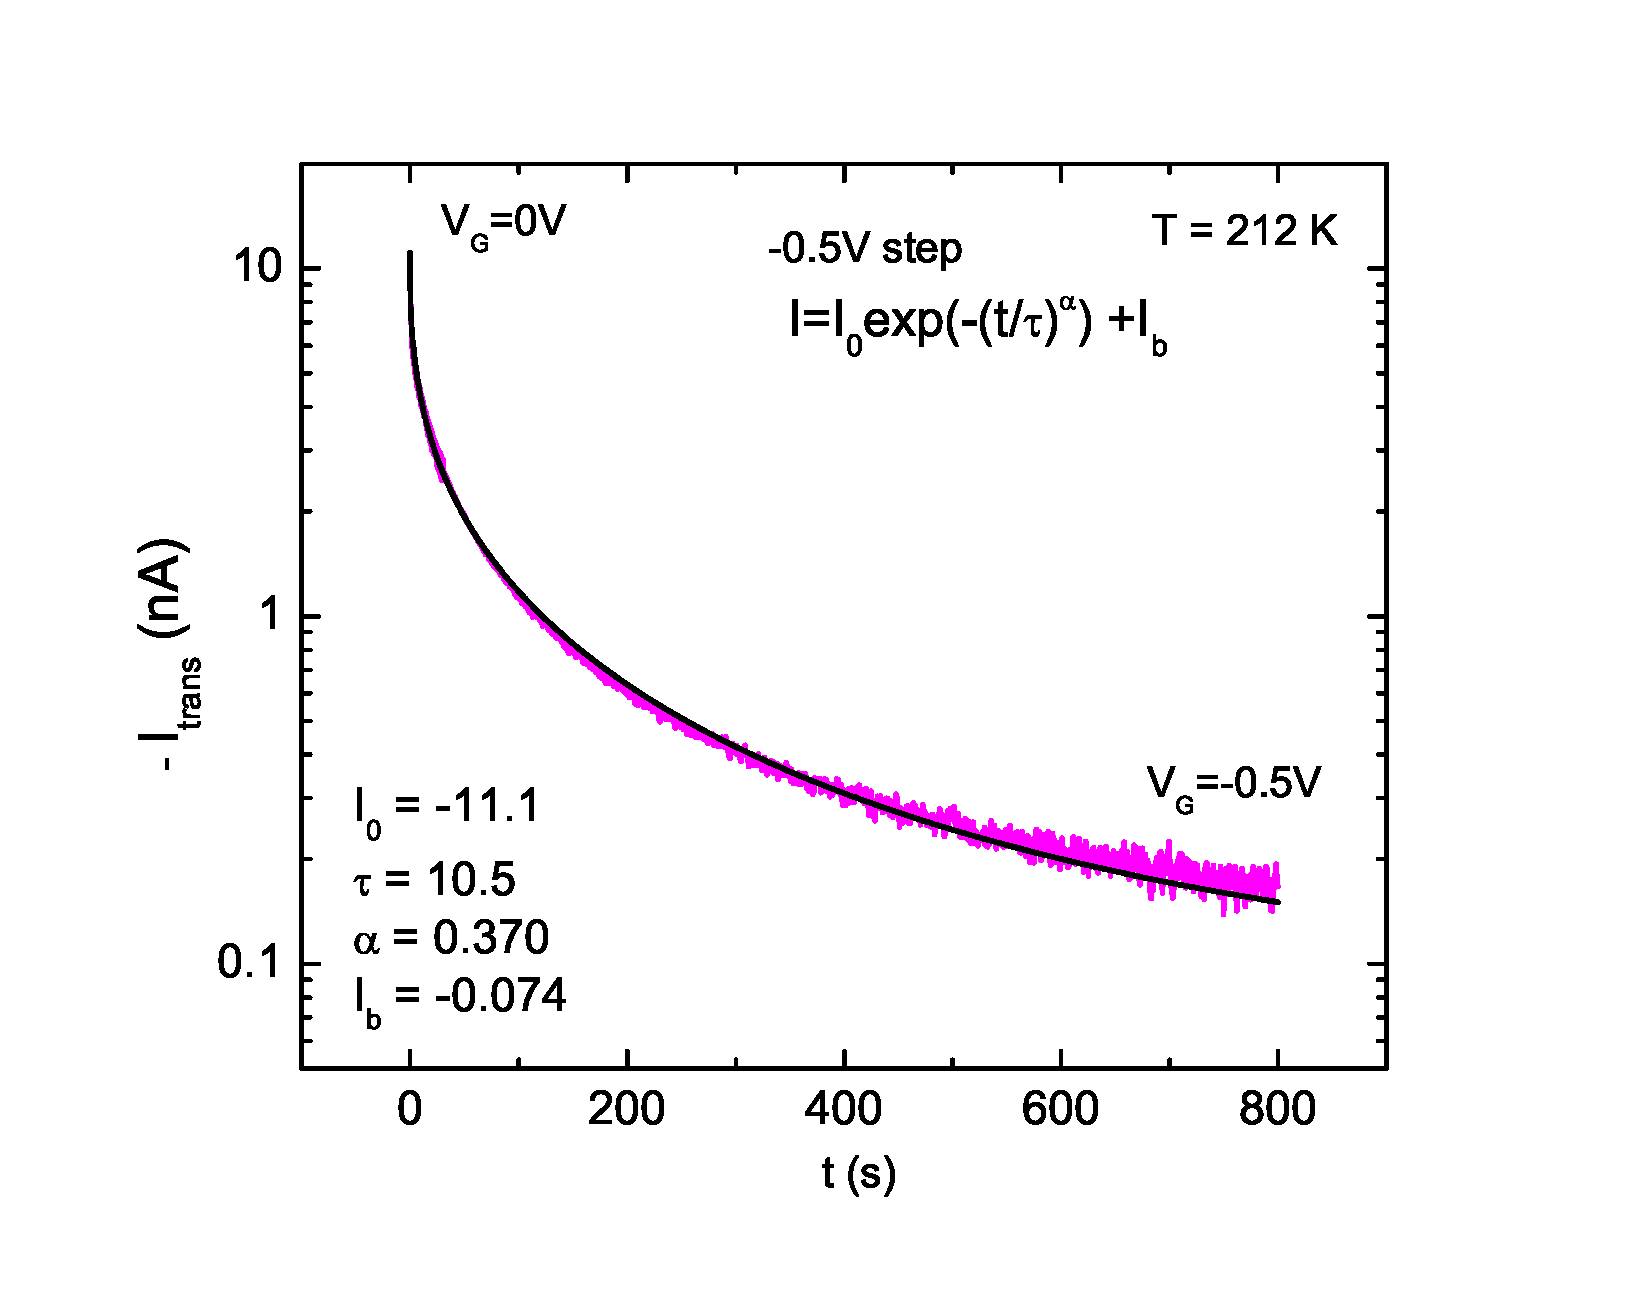
\includegraphics[width=0.65\linewidth]{ch-appendicies/figures/FigTransCurrent.eps}
\caption{\label{figtrans} 
The transient (discharging) current $I_{trans}$ versus time $t$ following a step-change of
$V_G$ from 0 to -5 V at $t$ = 0 at $T$ = 212 K in Sample 3. The observed current fits well to the stretched exponential form
Eq. \ref{Itrans} with the parameters $I_0$ = -11.1 nA, $I_b$ = -0.074 nA, $\alpha$ = 0.37, and $\tau$ = 10.5 s.
$I_b$ is the long-term steady-state background current. 
}
  \end{center}
\end{figure} 


%%%%%%%%%%%%%%%%%%%%%%%%%%%%%%%%%%
%%%%%%%%%%%%%%%%%%%%%%%%%%%%%%%%%%
%%%%%%%%%%%%%%%%%%%%%%%%%%%%%%%%%% FIGURE A2
\begin{figure}[!htbp]
  \begin{center}
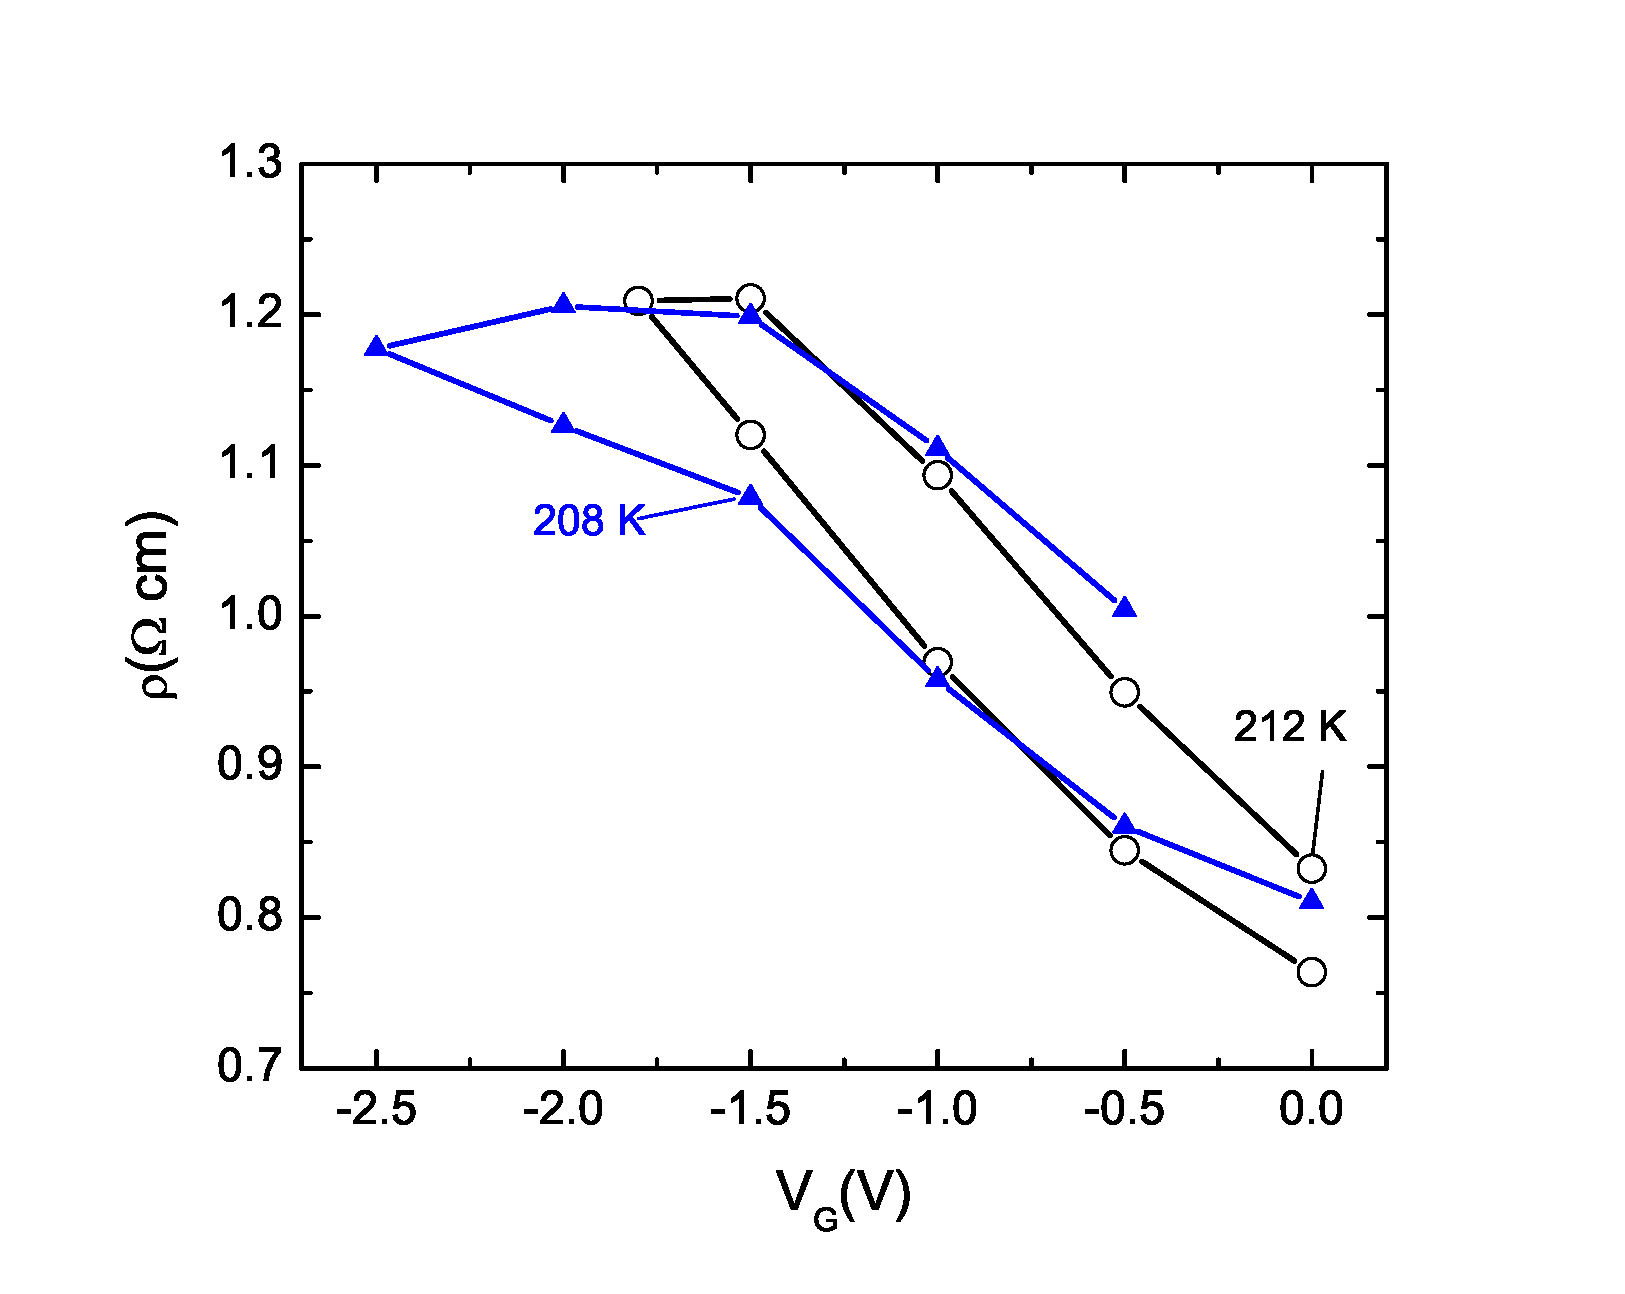
\includegraphics[width=0.7\linewidth]{ch-appendicies/figures/FigRvsVGLowT.eps}
\caption{\label{figRLowT} (color online) 
Apparent hysteretic behavior of $\rho$ vs. $V_G$ observed at temperatures close to the glass transition $T_G$. 
When the gating $T$ is too close to $T_G$, the background quasi-steady state $I_1$ and 
possibilities of chemical reaction are strong suppressed. However, at these temperatures, the ions are almost frozen and it may take a longer time for them to move back. Thus it leads to increased hysteresis in $\rho$ when $V_G$ is cycled (here $T$ = 208 and 212 K). The Hall density $n_H$ shows similarly large hysteresis (not shown). 
As discussed in the text, we show that this apparent low-temperature hysteresis results from incomplete
melting of the ionic liquid.
}
  \end{center}
\end{figure} 



%%%%%%%%%%%%%%%%%%%%%%%%%%%%%%%%%%
%%%%%%%%%%%%%%%%%%%%%%%%%%%%%%%%%%
%%%%%%%%%%%%%%%%%%%%%%%%%%%%%%%%%% FIGURE A3
\begin{figure}[!htbp]
  \begin{center}
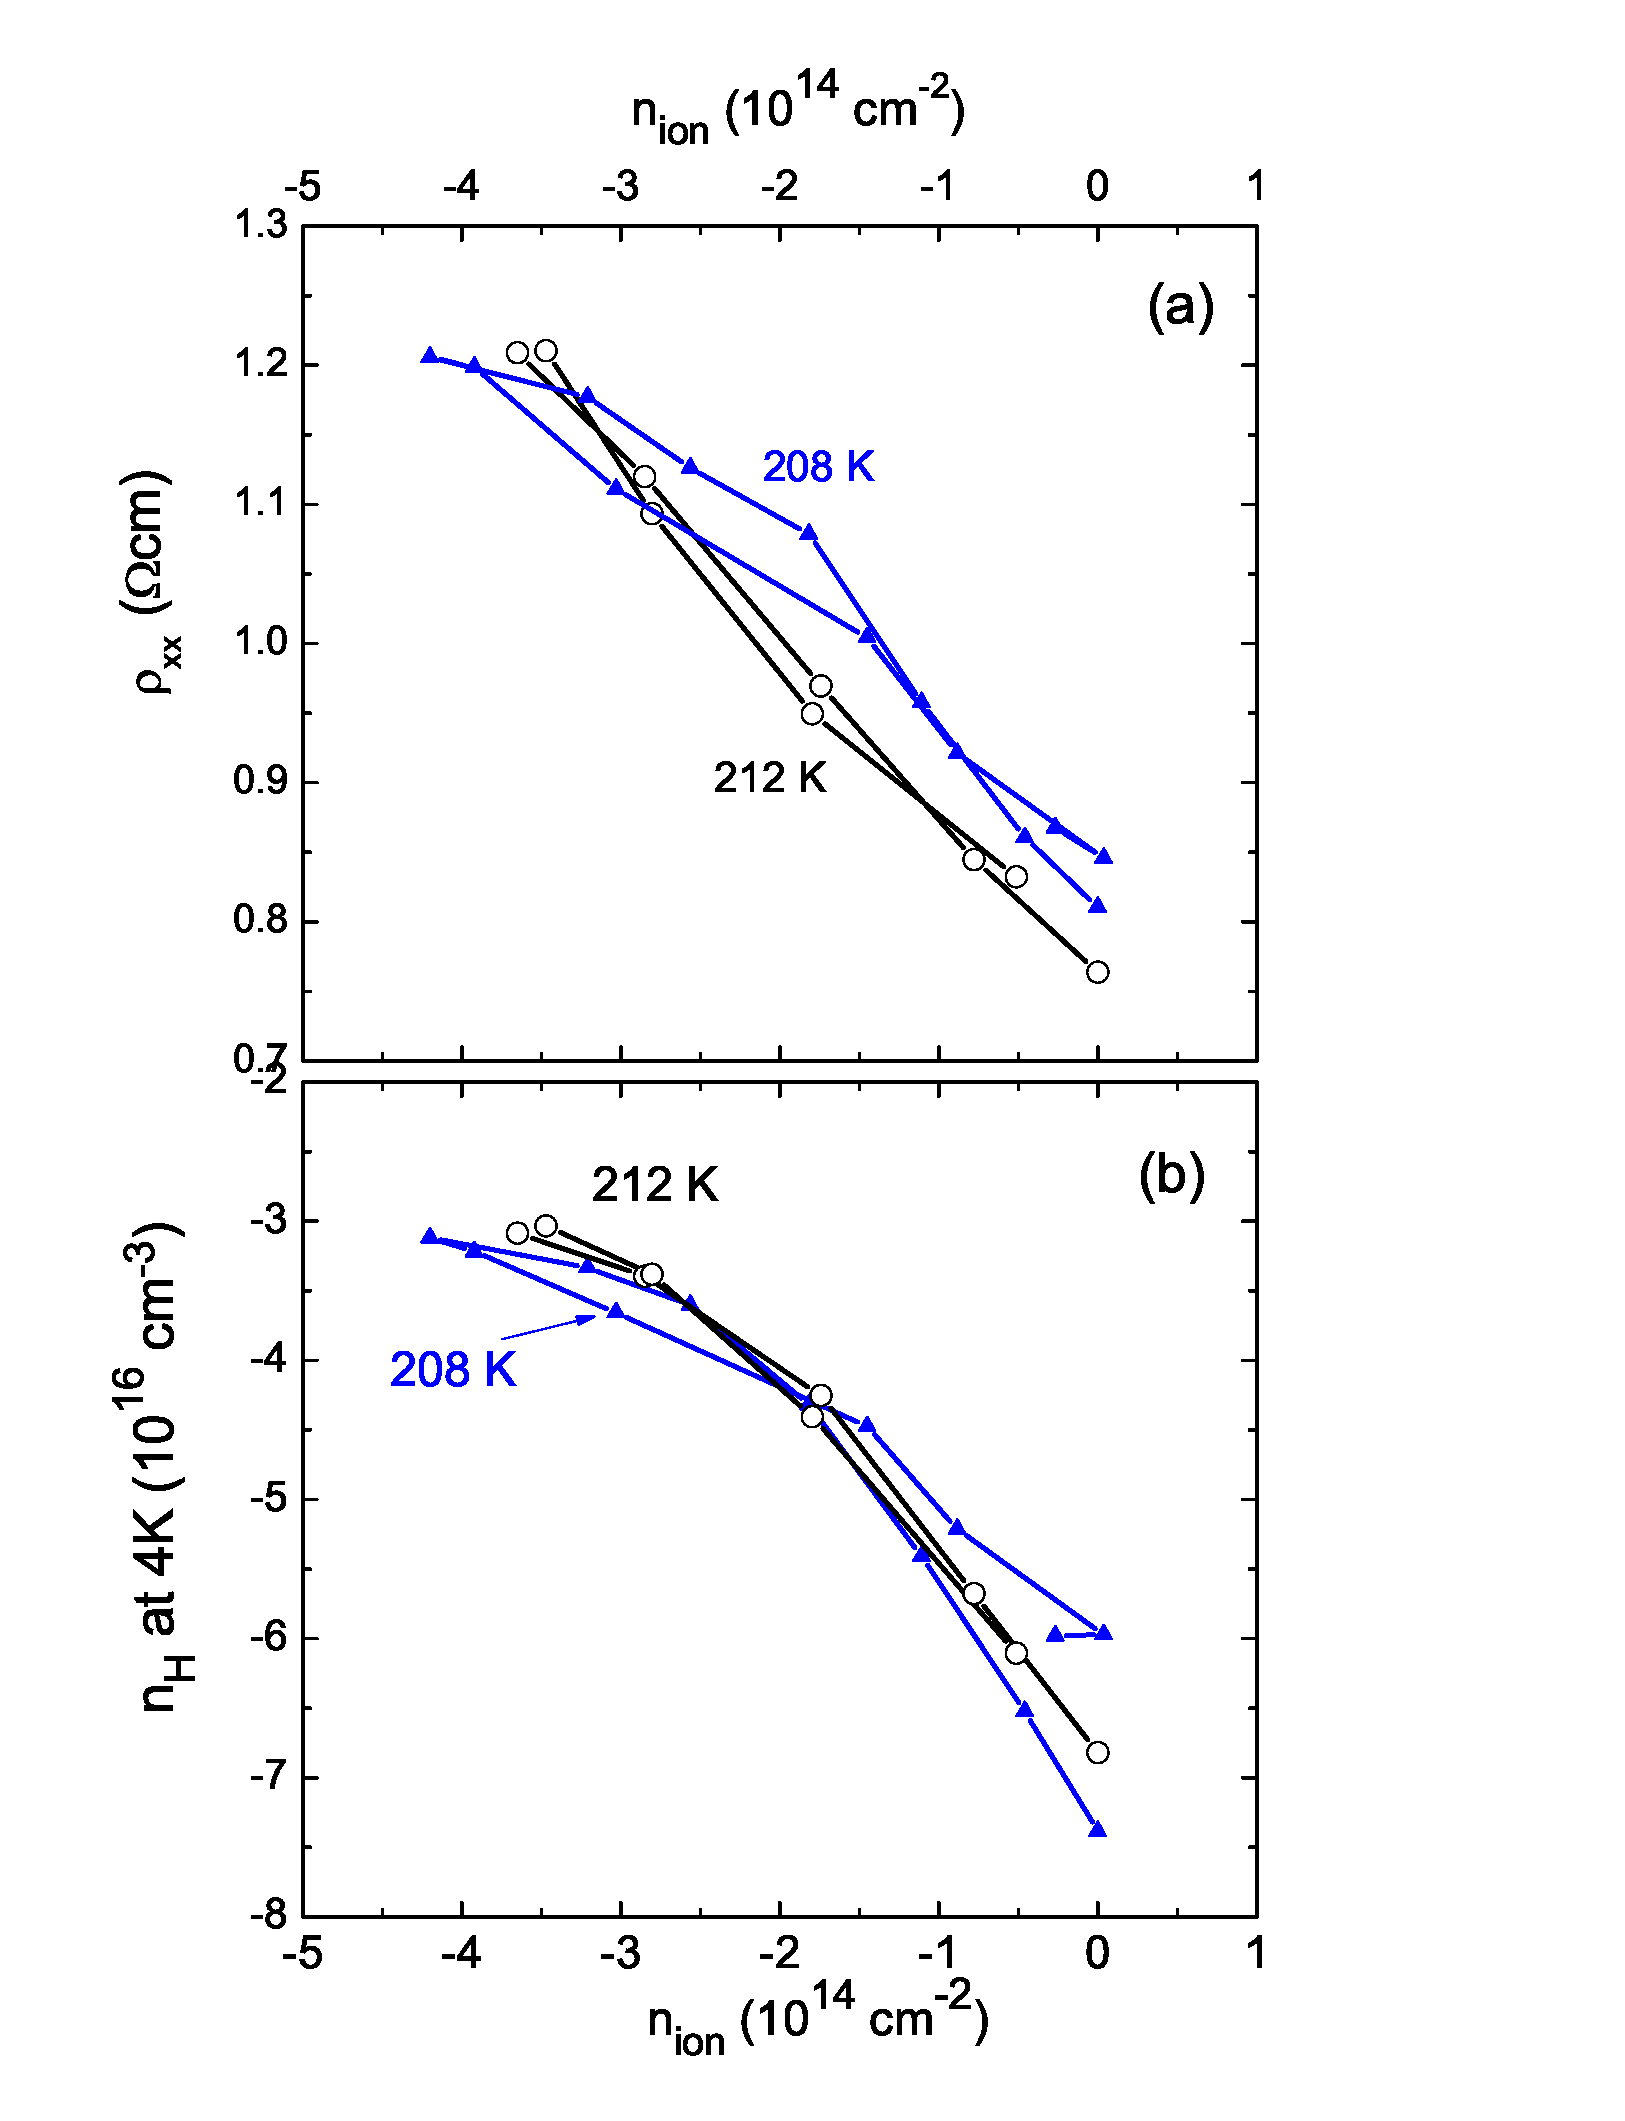
\includegraphics[width=0.7\linewidth]{ch-appendicies/figures/FigRvsNion.eps}
\caption{\label{figNion} (color online) 
Absence of low-temperature hysteresis when $\rho$ and $n_H$ are plotted against $n_{ion}=Q/eA$ (with $A$ = 2.9 mm$^2$), the accumulated charge calculated from the transient charging current.
Replotting the data for $\rho$ in Fig. \ref{figRLowT} versus $n_{ion}$ (instead of $V_G$) removes the hysteresis apparent in Fig. \ref{figRLowT}.
The difference indicates that the hysteretic behavior arises from the variation of $Q$ vs. $V_G$. A possible explanation is that it's hard for the ions to return when they are almost frozen. This figure shows that physically relevant quantities inside the
crystal $\rho$ and $n_H$ are dependent only on $Q$, the accumulated charge in the capacitor. It strongly supports the premise that band-bending 
produces the changes in sample conductance rather than chemical reaction.}
  \end{center}
\end{figure} 




Figure \ref{figRLowT} presents the changes in $\rho$ (Sample 3) as  $V_G$ is cycled between 0 and -2.5 V at 
low temperatures (208 and 212 K) that are close to the glass transition temperature $T_G$. In contrast to Fig. \ref{RvsVG}, we observe
sizeable hysteretic behavior (also in $n_H$, not shown). To show that this is not caused by
chemical reaction (which should be greatly suppressed at low $T$), we have measured the accumulated
$Q(t)$ and found that it displays the same hysteresis (vs. $V_G$). When we plot the changes
in $\rho$ and $n_H$ against $n_{ion} = Q/eA$ (see Fig. \ref{figNion}), 
the hysteretic behavior apparent in Fig. \ref{figRLowT} is largely removed.

This implies that, at these low $T$, a significant portion of the ionic ``solid'' accumulated at the
previous value of $V_G$ fails to melt and flow in response to the new $V_G$. Hence
$Q(t)$ never attains its equilibrium value even at long $t$. This leads 
to strong hysteresis in $Q$ vs. $V_G$. However,
the near-absence of hysteresis in Fig. \ref{figNion} shows that $\rho$ and $n_H$ adjust reversibly to
the non-equilibrium value of $Q$. The key parameter that
causes $\rho$ and $n_H$ to change is the electric-field $E(0^-)$ produced by $Q$ even when it lags
the applied $V_G$. This direct link provides further support for our conclusion that
the dominant effect of changing $Q$ is band-bending instead of chemical reactions.




